% $Author: predrag $ $Date: 2015-09-26 19:42:18 -0400 (Sat, 26 Sep 2015) $
% http://www.cns.gatech.edu/~predrag/papers/FoxCvi14.pdf

% elton/FoxCvi14/FoxCvi14.tex    pdflatex FoxCvi14
%     then:    pdflatex FoxCvi14; bibtex FoxCvi14; pdflatex FoxCvi14; pdflatex FoxCvi14
% for public version, toggle \draftfalse in setupFoxCvi14.tex
%     (that removes all comments, the blog)

\documentclass[aip,cha,reprint,
secnumarabic,
nofootinbib, tightenlines,
nobibnotes, showkeys, showpacs,
groupedaddress
%preprint,%
%author-year,%
%author-numerical,%
]{revtex4-1}
% aip,cha,preprint,numerical, nofootinbib,
% You should use BibTeX and apsrev.bst for references
% Choosing a journal automatically selects the correct APS
% BibTeX style file (bst file), so only uncomment the line
% below if necessary.
%\bibliographystyle{apsrev4-1}

        \input setupFoxCvi14
        \input ../inputs/def
        \input defFoxCvi14

\begin{document}

\title[Life \& Death]
{A Brief Life and Death of a Torus:
Computation of Quasiperiodic Solutions to the Kuramoto-Sivashinsky
Equation}

\author{Adam M. Fox}
\email{adam.fox@wne.edu.}
\affiliation{Department of Mathematics,
            Western New England University, Springfield, MA 01119 USA}
\date{\today}
%\date{July 19, 2012}
%\setcounter{page}{1}

    \begin{abstract}
The \KSe\ (KSE) arises in the study of
interfacial instability in a variety of settings such as flame-front
propagation and the liquid film on an inclined plane.  When only a single
spatial dimension is considered the system can be parameterized by the
length of the corresponding interval.  As the spatial domain increases,
the orbits of the \KS\ system become increasingly
turbulent.  Quasiperiodic solutions are theorized to exist within this
turbulence.  These solutions lie on invariant tori which act as barriers
to transport and are therefore of significant dynamical importance.
We will present a numerical method to compute such orbits and
describe their dynamics.
    \end{abstract}

\maketitle

\section{Introduction}
\label{s:intro}
Predicting the behavior of turbulent flows is exceptionally difficult.
Analysis of the topologically invariant structures, as
well as their stable and unstable manifolds, has proven fruitful in
gaining insight into the dynamics of such
systems.\rf{Christiansen:97,science04}  The earliest studies focused on
the simplest of such structures, namely the 0-dimensional \eqva.  Later
work extended these ideas to periodic orbits,\rf{lanVar1,SCD07}
topologically 1-tori, and, to a lesser degree, quasi-periodic
orbits,\rf{LCC06} which lie on higher dimensional tori.

In this paper we seek to further understand the role higher dimensional
tori play in the dynamics of infinite dimensional chaotic dynamical systems.
We study a quasi-periodic orbit that lies on a 2-torus in the
Kuramoto-Sivashinsky system parameterized by the system size $L$.  We
show that such a 2-torus can come into existence when a nearby stable
\po\ undergoes Hopf bifurcation and is later destroyed when it collides
with an unstable \po.  Unlike traditional KAM tori, this partially
hyperbolic torus does not appear to be vulnerable to resonances.

In \refsect{s:KSSys} we introduce the \KSe\ and describe its utility in
studying more general chaotic flows.  We then present variational methods
to compute periodic orbits and invariant tori in \refsect{s:Numerics},
first developed by Lan et al.  We apply these methods to study the birth,
life, and death of an invariant torus in \refsect{s:Life}.

\section{The \KSe}
\label{s:KSSys}
The \KSe\ \rf{ku,siv,Holmes96} is a simple yet physically intersesting nonlinear system that provides a foundation to study turbulence in more complex flows \rf{Holmes96}.   We will explore this system
parametrized by the system size $L$,
\beq
u_t=(u^2)_x-u_{xx}- u_{xxxx}
    \,,\qquad       x \in [0,L]
\,.
\ee{eq:kseq}
Following \refref{LCC06} we will restrict our study to the antisymmetric solution space of
\refeq{eq:kseq} with periodic boundary conditions, i.e.\ $u(-x,t)=-u(x,t)$
and $u(x+L,t)=u(x,t)$,
with $u(x,t)$ Fourier-expanded as
 \begin{equation}
u(x,t)=\sum_{k=-\infty}^{\infty} i a_k e^{ikqx}, \label{eq:uexpan}
\end{equation}
 where $q=2\pi/L$ is the basic wavenumber and
 $a_{-k}=-a_k \in \mathbb{R}$.  Accordingly, \refeq{eq:kseq} becomes
a set of ordinary differential equations~:
 \begin{equation}
\dot{a}_k=((kq)^2-
    (kq)^4)a_k - kq \sum_{m=-\infty}^{\infty} a_m a_{k-m}
\,.
\label{ksexpan}
\end{equation}
In the long-time limit of \refeq{ksexpan} for $k$ large $a_k$'s decay
faster than exponentially, so a finite number of $a_k$'s yields an
accurate representation of the long-time dynamics.  Previous
studies\rf{Christiansen:97,LCC06,lanVar1,SCD07} have shown that a truncation at $k=16$ is
sufficient for a quantitatively accurate calculation for the range of parameters that we are interested in.

\section{Numerical Methods} \label{s:Numerics}

\subsection{Preliminaries}
Here we describe a variational method to compute both periodic orbits
\rf{lanVar1} and invariant tori\rf{LCC06} in flows and maps of arbitrary
dimension.  Our presentation of these methods will be brief and we refer
the reader to the original articles for a more detailed discussion. Since
our primary goal is to examine the behavior of the \KSe\ we will restrict
our presentation of this method to the continuous time case.  We refer to
reader to the original articles for details on the application of this
technique to maps.

Let $\mathcal{M} \subset \mathbb{R}^d$ and $ x \in \mathcal{M}$.  We seek to compute periodic orbits and invariant tori of flows defined by first order ordinary differential equations
\begin{equation}
 \frac{d x}{dt}= v( x).
\,
\label{ODEs}
\end{equation}
For simplicity, we assume that the vector field $ v( x)$ is sufficiently smooth.

The variational technique has the same basic approach for computing tori
and periodic orbits.  We begin with some initial guess $ x(s,\tau)$ where
$s$ is a cyclic variable that parameterizes a loop.  The variable
$\tau$ acts as a ``fictitious time'' and parametrizes a continuous family
of  guess loops, with the initial guess at $\tau=0$ and the true, desired
orbit at $\tau=\infty$.  In the following sections we derive the
evolution rule of the loop under $\tau$ for the two cases.

\subsection{Computation of Periodic Orbits}

Let $f$ be the flow of \refeq{ODEs}, that is $ \frac{d}{dt}f^{t}(x)=v(x)$. A periodic orbit is determined by a pair $(x,T)$, with $ x \in
\mathcal{M}$ and $T \in \mathbb{R}$, such that
\[
 f^T( x)= x.
 \]
We parameterize an initial guess for such an orbit
$\tilde{x}_n=\tilde{x}(s_n,0)$, with $\{s_0,s_1,\cdots,s_N\}\in[0,2\pi]$,
such that $\tilde{x}(s,0)=\tilde{x}(s+2\pi,0)$.  For simplicity we choose an
evenly spaced grid, $\Delta s=2\pi/N$.  We define the $s$-velocity
$\tilde{v}$ as the derivative of this loop with respect to $s$,
\begin{equation}
 \frac{d \tilde{x}}{ds}=\tilde{v}( \tilde{x}).
\,
\label{Svel}
\end{equation}

The fundamental idea of this algorithm is that for any periodic loop the
flow velocity must equal the $s$-velocity up to some constant, i.e.
$\tilde{v}( \tilde{x})=\lambda  {v}(\tilde{x})$. The local time scaling
factor
\begin{equation}
\lambda=\Delta t / \Delta s,
\label{lam}
\end{equation}
where $\Delta t = T/N$, serves to match the magnitudes of these tangents.

We must now construct a rule such that our initial guess loop
$\tilde{x}(s,0)$ approaches a periodic orbit as $\tau \to \infty$.  Let
$x(t)=f^t(x)$ be the state of the system at time $t$ and
$J(x,t)=dx(t)/dx(0)$ be the corresponding Jacobian matrix.  We compute
this matrix by simultaneously integrating the system \refeq{ODEs} and
\begin{equation}
\frac{dJ}{dt}=AJ, \; A_{ij}=\frac{\partial v_i}{\partial x_j}, \; \mbox{ where } J(x,0)=Id\,
\label{Jacobian}
\end{equation}

We assume our initial guess is close to a true periodic orbit, $x_n = \tilde{x}_n+\delta\tilde{x}_n$, so that
\[
f^{\Delta t + \delta t_n}(\tilde{x}_n+\delta\tilde{x}_n)=\tilde{x}_{n+1}+\delta\tilde{x}_{n+1}
\]
Linearizing about $\tilde{x}_n$ and $\Delta t$ yields
\[
f^{\delta t}(x) \approx x+v(x)\delta t, \hfill f^t(x+\delta x)\approx x(t)+J(x,t)\delta x.
\]
We can use these linearizations to construct the multiple-shooting Newton-Raphson equation
\begin{equation}
\delta \tilde{x}_{n+1}-J(\tilde{x}_n,\Delta t) \delta \tilde{x}_n - v(\tilde{x}_n)\delta t_n = f^{\Delta t}(\tilde{x}_n)-\tilde{x}_{n+1}. \label{NReq}
\end{equation}
Lan et al\rf{lanVar1} showed  that this Newton-Raphson iteration generates a sequence of loops with a decreasing cost function provided the initial guess is sufficiently close to the true periodic orbit.

We now iterate the system by $\delta\tau$, or, equivalently, multiply the right hand side of \refeq{NReq} by $\delta\tau$.  We can simplify the result by noting
\begin{align}
\delta t_n&=\frac{\partial \lambda}{\partial \tau}(s_n,\tau)\delta\tau\Delta s \; \mbox{    from \refeq{lam} and} \\
\delta\tilde{x}_n&=\frac{\partial}{\partial \tau}\tilde{x}(s_n,\tau)\delta\tau.
\end{align}
Dividing both sides of \refeq{NReq} by $\delta\tau$ thereby yields
\begin{align}
\frac{d\tilde{x}_{n+1}}{d\tau}-J(\tilde{x}_n,\Delta t)\frac{d\tilde{x}_n}{d\tau}&-v_{n+1}\frac{\partial \lambda}{\partial \tau}(s_n,\tau)\Delta s \nonumber \\
&=f^{\Delta t}(\tilde{x}_n)-\tilde{x}_{n+1}.
\label{SimpNR}
\end{align}

Now, in the limit as $N\to\infty$ both $\Delta s$ and $\Delta t$ approach
zero.  This gives the estimates
\begin{align}
v_{n+1} &\approx v_{n}, \hspace{20mm} f^{\Delta t}(\tilde{x}_n)\approx\tilde{x}_n+v_n\Delta t. \nonumber\\
\tilde{x}_{n+1}&\approx\tilde{x}_n+\tilde{v}_n\Delta s, \hspace{7mm} J(\tilde{x}_n,\Delta t)\approx 1+A(\tilde{x}_n)\Delta t \nonumber
\end{align}
These approximations along with \refeq{lam} yield the result
\begin{equation}
\frac{\partial^2\tilde{x}}{\partial s \partial \tau}-\lambda A\frac{\partial \tilde{x}}{\partial \tau}-v\frac{\partial \lambda}{\partial\tau}=\lambda v-\tilde{v}
\label{POEqn}
\end{equation}
This evolution equation describes the deformation of the
initial guess loop $\tilde{x}$ to the true periodic orbit $x$.

For the discretized loop $\tilde{x}_n$ we approximate the $s$-derivative
using a standard four-point approximation, $\tilde{v}_n=\frac{\partial
\tilde{x}}{\partial s} \approx  (D\tilde{x})_n$, where $D$ is a
block-diagonal matrix, see \refref{lanVar1} for details.  The evolution
equation \refeq{POEqn} of the discretized system is then
\begin{equation}
\begin{pmatrix} \hat{A} & \hat{v} \\ \hat{r} & 0 \end{pmatrix}
    \begin{pmatrix} \delta\hat{x} \\ \delta\lambda \end{pmatrix}
    =\delta\tau  \begin{pmatrix} \lambda\hat{v}-\hat{\tilde{v}} \\ 0 \end{pmatrix},
\label{POEqnDisc}
\end{equation}
where $\hat{A}=D-\lambda\mbox{diag}[A_1,A_2,\cdots,A_N]$, $A_n=A(\tilde{x}(s_n))$, and
\begin{align}
\hat{v} &=(v_1,v_2,\cdots,v_N), \; v_n=v(\tilde{x}(s_n)),\\
\hat{\tilde{v}} &=(\tilde{v}_1,\tilde{v}_2,\cdots,\tilde{v}_N), \;  \tilde{v}_n=\tilde{v}(\tilde{x}(s_n))
\nonumber
\end{align}
are the vector fields whose direction we wish to coincide.  The parameter $\delta\tau$ is the Euler step size used to solve the fictitious-time differential equation.

The $Nd$ dimensional vector $\hat{r}$ imposes a constraint on the coordinate variations
$\delta \hat{x}=(\delta\tilde{x}_1,\delta\tilde{x}_2,\cdots,\delta\tilde{x}_N)$.  Note that every periodic orbit remains a periodic orbit under a cyclic permutation of its discretized points.  The operation
\[
\overline{A}=\frac{\partial}{\partial s} - \lambda A
\]
used in \refeq{POEqn} therefore has a marginal eigenvector $v(\tilde{x}(s))$ with zero eigenvalue.  As we discuss below, the parameter $\lambda$ is fixed in our implementation.  Therefore, as $\tau \to \infty$,
\[
 \overline{A}\frac{\partial x}{\partial \tau}=0
 \]
so $\overline{A}$ becomes singular and numerical issues arise.  We remedy
this problem by fixing the first coordinate of the first point of the
discretized orbit $\tilde{x}_1(s_1,\tau)=const$.  The vector $\hat{r}$
ensures this point is fixed.

\subsection{Implementation of the Algorithm}

The first step in implementing this algorithm is choosing an appropriate
guess loop. There are a variety of effective shooting methods that can be
employed when attempting to compute an unstable or nonattracting stable
periodic orbit, see \refref{SCD07} for examples.  When computing
attracting periodic orbits, such as those shown below, one can simply
iterate a random orbit until it becomes sufficiently close to the
attracting orbit and then use the result as the initial guess.  This is
the approach we used.

We employed a 256-point discretization for the loop $\tilde{a}_n$ (note
that we now use $a$ rather than $x$ for the system \refeq{ksexpan}).  The
first point of this discretization was chosen on the \PoincSec\
$a_1=0.06$ and this point was evolved using \refeq{ksexpan} until the
orbit returned to the $a_1=0.06$ section at time $T_f$.  We then selected
256 points evenly spaced on the orbit so $\Delta t= T_f/256$ and $\Delta
s=2\pi/256$.  The loop was then evolved using \refeq{POEqnDisc} and
$\delta\tau=1$ until the error $||\lambda v- \tilde{v}||_{2} \leq
10^{-12}$.  It is important to note that the error in this calculation is
not the same at the error in the periodic orbit, ie $||  f^T(a)- a ||_2$.

An initial condition for the periodic orbit shown in \reffig{fig:POrbit}
was generated by evolving a randomly selected point in the neighborhood
as described above. The initial error $||\lambda v- \tilde{v}||_{2}
\approx 8.63 \times 10^{-4}$.  This error dropped to $5.62 \times
10^{-11}$ after one iteration and $2.73\times 10^{-14}$ after a second.
The final error in the periodic orbit $||  f^T(a)- a ||_2=9.94\times10^{-7}$.
This error could be reduced by increasing the number of points used in
the discretization.  The algorithm required approximately 20 seconds
running on Matlab %R2014b
on a MacBook Pro laptop.
% with 3.06 GHz Intel Core 2 Duo processor and 8GB of memory.

When the algorithm converged successfully at fixed $L$ we used the result
as the initial guess for the periodic orbits at nearby values of $L$.  A
more sophisticated extrapolation scheme may be more effective however we
found the algorithm to be robust enough that it wasn't necessary.

 \begin{figure}[!h]
\centering
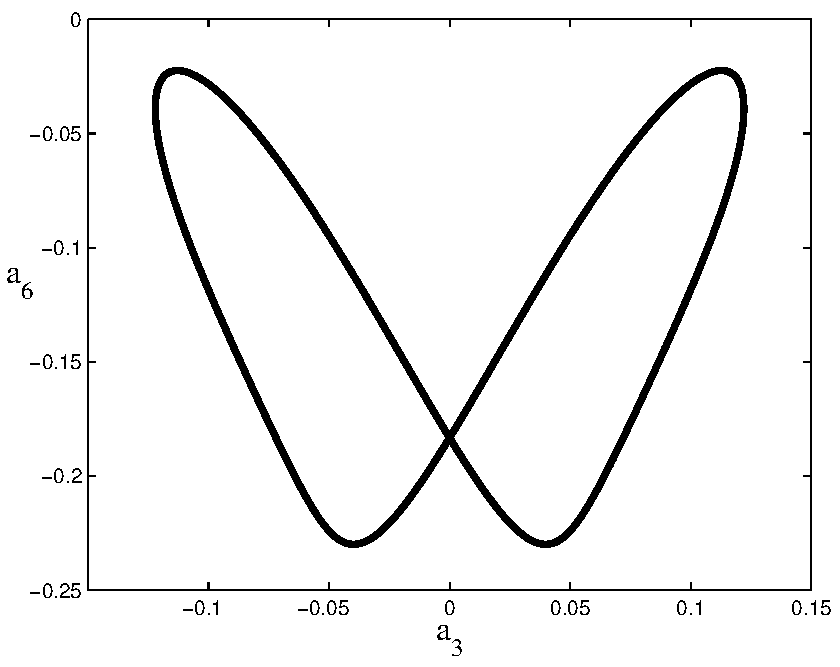
\includegraphics[width=3in]{PO1_L41p2}
  \caption{
 A projection of a periodic orbit of the \KSe\ for $L=41.2$.  The return time is $T \approx 24.11$.
   }
  \label{fig:POrbit}
 \end{figure}



\subsubsection{Stability of Periodic Orbits in the Kuramoto-Sivashinsky System}

Our discretization of the \KS\ equation is 16-dimensional, so the linear
stability of an orbit is described by the 16 eigenvalues $\ExpaEig_j$ of
its Jacobian matrix \refeq{Jacobian}.  If the orbit is periodic, the
Floquet multiplier corresponding to perturbations along the orbit is
unity. The observed periodic orbits of the \KSe\ have a few relatively
large leading multipliers but the majority are strongly contracting,
$|\ExpaEig_j| <10^{-2}$ or less.  These strongly contracting multipliers
play a relatively insignificant role in guiding the overall dynamics.  We
will be primarily concerned with those few directions for which the
magnitude of Floquet multipliers is relatively large, i.e. $|\ExpaEig_j| >10^{-2}$.


\subsection{Computation of Invariant Tori}

Lan\rf{LCC06} demonstrated the existence of an invariant two-torus in the
\KSe\ .  To compute this torus we employ the \emph{ \PoincSec\ } method.  In
this method, one records the coordinates $\sspRed_n$ of the trajectory
$\ssp(t)$ at the instants $t_n$ when it traverses a fixed oriented
hypersurface $\PoincS$ of codimension 1. For the high\dmn\
Kuramoto-Sivashinsky flow, the practical choice is a hyperplane.

The application of the \PoincSec\ method transforms the problem
from computing a $2$-torus in a continuous system to the computation of a
$1$-torus in a discrete one.  A $1$-dimensional torus is a closed loop on
$\PoincS$ which is invariant under the Poincar\'e map.  We parameterize
this loop $x(s)$ with $s\in[0,2\pi)$ such that $ x (s)= x (s+2\pi)$.  The
dynamics on the tori that we will examine are conjugate to a rigid
rotation, that is
\begin{equation}
 g( x(s)) =  x(s+\omega)
\,,
\label{torusMap}
\end{equation}
where $g$ is the Poincar\'e return map and $\omega \in \mathbb{R}$ is the \emph{rotation number}.

The initial guess loop $x(s,0)$ is discretized by $N$ points of dimension
$k$ that lie on $\PoincS$. We construct a system of ODEs in $\tau$ such
that the error
\[
F(s,\tau)=g(x(s,\tau))-x(s+\omega(\tau),\tau)
\]
goes to zero as $\tau \to \infty$.  Note here that the shift $\omega$ may
also evolve with $\tau$.  There are many choices one may make in this
construction.  We make the simple choice,
\[
\frac{dF}{d\tau}=-F
\]
yielding the differential equations
\begin{align}
&\frac{\partial x}{\partial \tau}(s+\omega(\tau),\tau)
+\frac{\partial x}{\partial s}(s+\omega(\tau),\tau)
\frac{\partial \omega}{\partial \tau}(\tau)  \nonumber \\
&-\tilde{J}(x(s,\tau))
\frac{\partial x}{\partial \tau}(s,\tau)=F(x(s,\tau))\nonumber
\end{align}
where $\tilde{J}$ is the Jacobian matrix of the Poincar\'e map $g$.  This
Jacobian is different than $J$, the Jacobian of the full system, however
we can easily find $\tilde{J}$ from $J$.\rf{DasBuch}  Let $x'=g(x)$ be the
first return to $\PoincS$ of $x\in\PoincS$, $v'=v(x')$, $U$ be a function
such that $U(x)=0$ whenever $x\in\PoincS$, and $U'=U(x')$.  The Jacobian
$\tilde{J}$ is then given by
\[
\tilde{J}_{ij} = (\delta_{ik}-\frac{v_i' \partial_kU'}{v'\cdot\partial U'})J_{kj}.
\]

If we are
searching for an invariant 1-torus of {a} given topology, the shift
$\omega=\omega(\tau)$ varies
with the fictitious time $\tau$, and
is to be determined simultaneously with the 1-torus itself.
Lan~\etal\rf{LCC06} impose the {\em phase condition}\rf{sh05fou}
\begin{equation}
\oint ds\!
    \left(
    v(s,\tau)  \cdot \frac{\partial x}{\partial \tau}(s,\tau)
    \right) =0
\,, \label{eq:nonsp1}
\end{equation}
 which ensures that during the fictitious time evolution
the average motion of the points along the
loop  equals zero. Empirically, for  this  global loop
constraint the fictitious time dynamics is more stable than
for a single-point constraint such as $\delta x(0,\tau)=0$.
For $m$-torus, $ v(s,\tau)$ is a $[d \times m]$ tensor and
\refeq{eq:nonsp1} yields $m$ constraints.


In practice, we expand $x$, $f(x)$, and the {\jacobianM} $\tilde{J}$ in terms of their Fourier series,
\begin{align}\label{eq:FExp}
x(s,\tau)&=\sum_{k} a_k(\tau) e^{i k s}\nonumber \\
g(x(s,\tau))&=\sum_{k} b_k(\tau) e^{i k s}\\
\tilde{J}(x(s,\tau))&=\sum_{k} \tilde{J}_k(\tau) e^{i k s} \nonumber
\end{align}
Using this representation the artificial-time ODEs become
\begin{equation}
\label{eq:Newton}
\left(\frac{da_k}{d\tau}+ika_k\frac{d\omega}{d\tau}\right)e^{ik\omega}-\sum_j \tilde{J}_{k-j}\frac{da_j}{d\tau}=b_k-a_ke^{ik\omega}
\end{equation}
and the phase condition \refeq{eq:nonsp1} is given by
\begin{equation}
\label{eq:PhaseCond}
\sum_k ka_k^* \frac{da_k}{d\tau} =0
\end{equation}
and is solved simultaneously with \refeq{eq:Newton}.  Solving this
$[(dN+1)\!\times\!(dN+1)]$ system is the most numerically intensive component of
the algorithm.  We employ the $LU$ factorization technique.

\subsection{Implementation of the Algorithm}
We first computed a torus at $L=41.10$ using an $N=16$ point discretization on the \PoincSec\ $a_1=0.06$ with an error threshold of $10^{-7}$.  An initial guess was generated by iterating a randomly chosen nearby point until it intersected \PoincSec\ $N$ times, ignoring the first few transient intersections that occur before the orbit has settled onto the attracting torus.   An initial estimate for the rotation number $\omega$ can be generated by minimizing the distance between the first return $x'$ of a point $x$ and the shift $x(s+\omega)$.  This processes yielded an approximation of $\omega \approx 0.12$.

The system of $dN+1$ ODEs given by  \refeq{eq:Newton} and \refeq{eq:PhaseCond} is solved using the simple forward Euler method with step size $1$.  The initial error $||F(s,\tau)||_2= 0.0016$ which fell to $||F(s,\tau)||_2= 2.28 \times 10^{-8}$ after 6 iterations using $\delta \tau = 1$ and requiring 82 seconds running on Matlab on a Macbook Pro.   This torus served as an initial guess for the torus at $L=41.11$.  In this case only 3 iterations and 47 seconds were required for convergence.  Linear extrapolation was used to generate an initial guess for the torus at $L=41.12$.  Only two iterations and 36 seconds were required for convergence.

Additional care is needed when computing the torus for smaller values of $L$.  As $L$ becomes smaller the torus grows and becomes less circular, see \reffig{fig:Tori}.  A larger discretization therefore becomes necessary to achieve the desired accuracy.  Whenever the algorithm failed to converge to the desired accuracy the number of points in the discretization was doubled.  This first occurred at $L=41.06$ when $N$ doubled to 32, and again at $L=40.90$.

 \begin{figure}[!h]
\centering
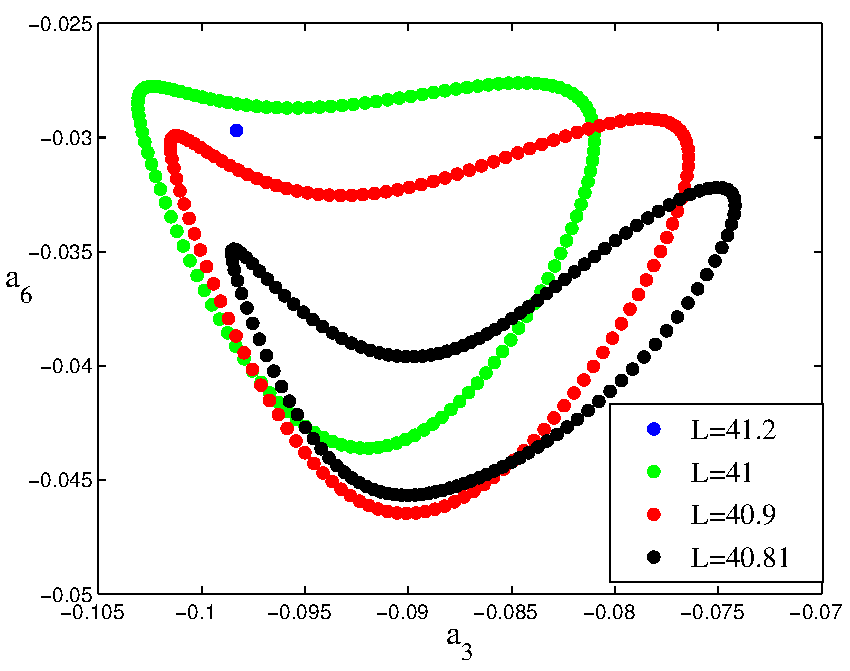
\includegraphics[width=3in]{KSTori}
  \caption{
 Projection of the invariant tori of the \KSe\ over a range of parameter values.}
  \label{fig:Tori}
 \end{figure}

\section{The life cycle of an invariant torus of the Kuramoto-Sivashinsky flow}
\label{s:Life}

When $L>42$ we do not observe any invariant tori, however periodic orbits
are abundant.  One such periodic orbit, the one shown in
\reffig{fig:POrbit}, has three leading multipliers other than the unity
multiplier: a single positive real multiplier less than one, and a complex pair
$\{\ExpaEig_{j},\ExpaEig_{j+1}\} =
\{\exp(\theta_j)|\ExpaEig_{j}|,\exp(-\theta_j)|\ExpaEig_{j}|\}$ with
moduli less then unity.  As $L$ decreases the moduli of these multipliers increase and,
 at $L \approx 41.95$, becomes one.  The resulting Hopf
bifurcation gives birth to an attractive two-torus, shown in
\reffig{fig:Tori}, analogous to the limit cycles seen in bifurcations of
\eqva.

As $L$ continues to decrease two significant phenomena occur.  First, the
invariant torus grows larger, as can be seen in \reffig{fig:Tori}.
Secondly, the periodic orbit contained within the torus undergoes an
additional bifurcation, see \reffig{fig:POBif}.  At $L \approx 40.84$ the
complex eigenvalues of the periodic orbit collide causing the orbit to
become unstable.  A new stable periodic orbit is also generated, see
\reffig{fig:POBif}.

Although the torus does grow as $L$ decreases it is still quite narrow even at its
largest.  Indeed, the quasi-periodic orbit on the torus and the periodic
orbit in the interior of the torus are visually indistinguishable.  It is
therefore unclear how dynamically important this particular torus is.

 \begin{figure}[!h]
\centering
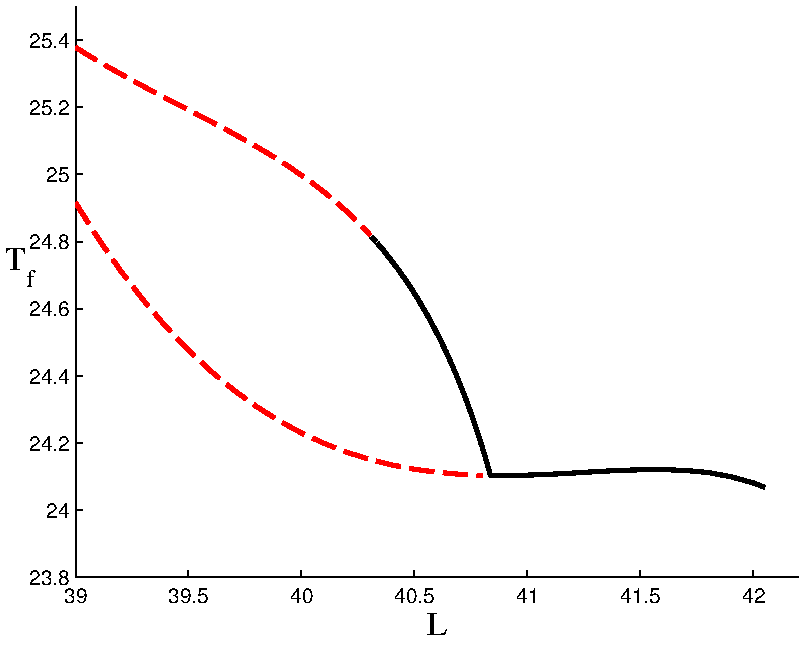
\includegraphics[width=3in]{POBif}
  \caption{
 Bifurcations diagram of the periodic orbits nearby the invariant torus.  The dashed red line indicates an unstable orbit while the solid black line indicates a stable orbit.
   }
  \label{fig:POBif}
 \end{figure}

 Previous studies of symplectic and volume-preserving systems have shown that the growth of a Sobolev seminorm can be used to predict the breakdown of tori \rf{Calleja10a,Calleja10b,Fox14}.  We define this seminorm as
\begin{equation}
 ||\overline{a}_k||_m^2 =  \sum_{j}(2\pi|j|)^{2m}|\overline{a}_k|^2
\,,
\label{Snorm}
\end{equation}
where $\overline{a}_k$ are the Fourier coefficients of the $k^{th}$ dimension of $a$.  A plot of $||\overline{a}_2||_3^2$ for $L$ near the destruction of the torus is shown in \reffig{fig:Snorm}.   The value of the seminorm appears to become infinite at a some critical value, $L_{cr}$.  At $L_{cr}$ the torus loses analyticity and, we assert, ceases to exist.  We can estimate $L_{cr}$ by modeling the data as a pole,
\begin{equation}
||\overline{a}_k||_m^2  \sim \frac{\alpha}{(L-L_{cr})^{\beta}} \, .
\label{eq:pole}
\end{equation}
A nonlinear least squares fit using the final 5 points gives $L_{cr} \approx 40.8027 \pm 4 \times 10^{-4}$.  This value was consistent for different values of $m$ and $k$ and number of points used.

 \begin{figure}[!h]
\centering
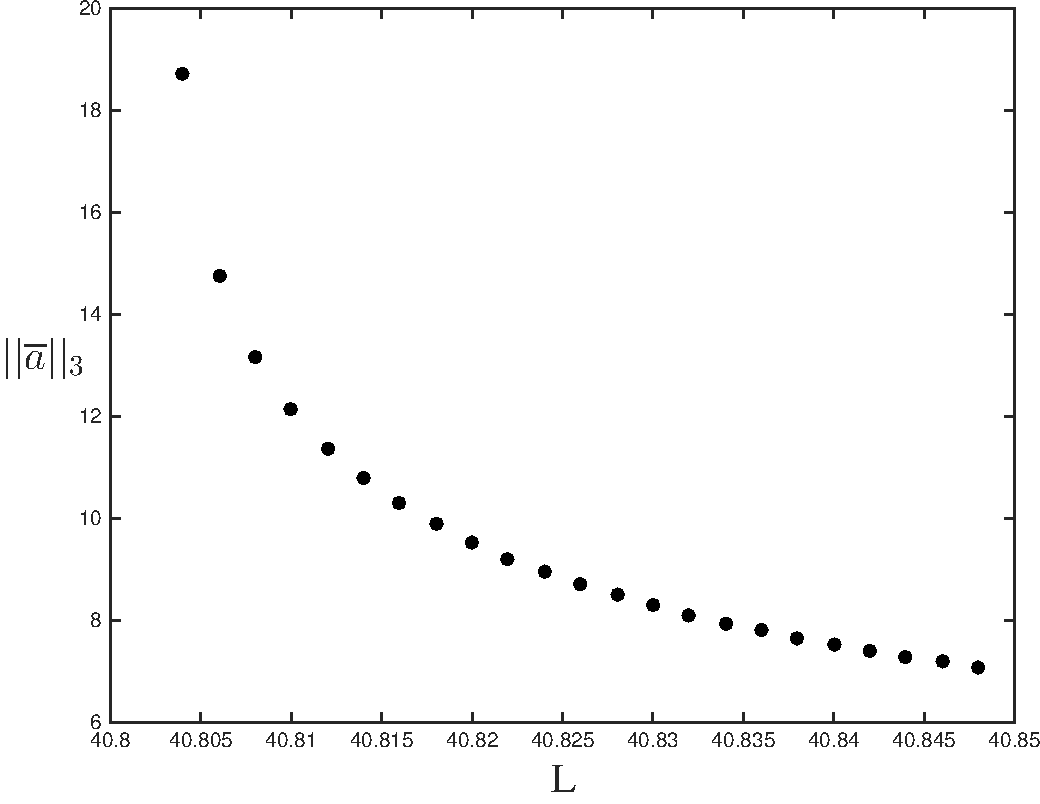
\includegraphics[width=3in]{KS_Snorm}
  \caption{
Values of the Sobolev seminorm \refeq{Snorm} with $m=3$ of the Fourier coefficients of $a_2$.  This norm becomes infinite at $L_{cr} \approx 40.8027 \pm 4 \times 10^{-4}$.
   }
  \label{fig:Snorm}
 \end{figure}

The destruction of the torus appears to be
caused by a collision between the torus and the periodic orbit shown in \reffig{fig:POrbit}, which is unstable for $L<40.84$, recall \reffig{fig:POBif}. To test this hypothesis we computed the minimum distance between the periodic orbit and the torus over a range $L$ values, see \reffig{fig:Collision}.  Specifically, we examined the distance on the $(a_3,a_6)$ projection on different Poincar\'e sections $a_1=const$ and found the minimum distance over all sections.  The 5 points closest to the collision were fitted to a pole, as in \refeq{eq:pole}, yielding an estimate of the collision parameter of
$
L_{cr}=40.8019 \pm 7 \times 10^{-4}
$.  The close agreement of this estimate to the one derived from the Sobolev norm provides strong numerical evidence of the validity of both techniques.

 \begin{figure}[!h]
\centering
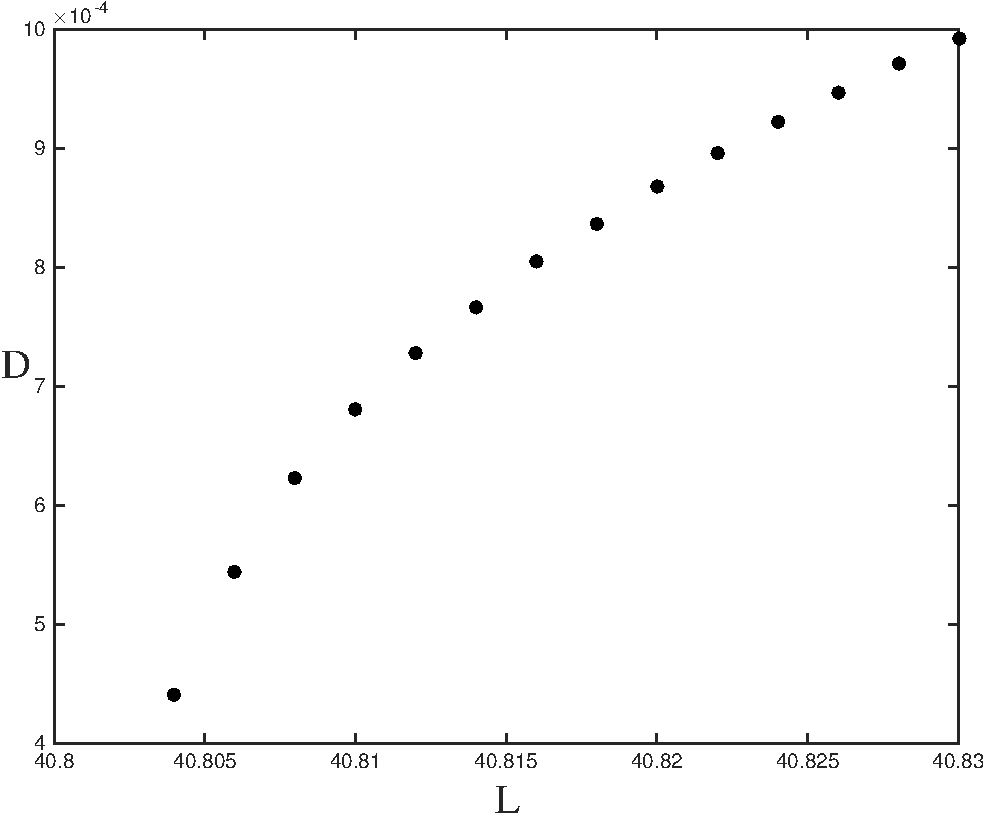
\includegraphics[width=3in]{POvsQPDist.pdf}
  \caption{
  Minimum distance between the unstable periodic orbit shown in \reffig{fig:POrbit} and the torus surrounding it.  The periodic orbit collides with the torus at $L_{cr}=40.8019 \pm 7 \times 10^{-4}$
   }
  \label{fig:Collision}
 \end{figure}

 \subsection{Rotation Numbers of the Invariant Tori}
The rotation number $\omega$ of the torus is fixed by the dynamics and determined by the phase condition \refeq{eq:PhaseCond}.  Unlike KAM tori, whose rotation numbers must be sufficiently irrational \rf{delaLlave01}, this partially hyperbolic torus does not exhibit any sensitivity to resonance, as shown in \reffig{fig:KSRotNums}.  Indeed, we examined the region near $\omega=\frac{1}{10}$ more closely and found no evidence that the torus was affected by the resonance.

 \begin{figure}[!h]
\centering
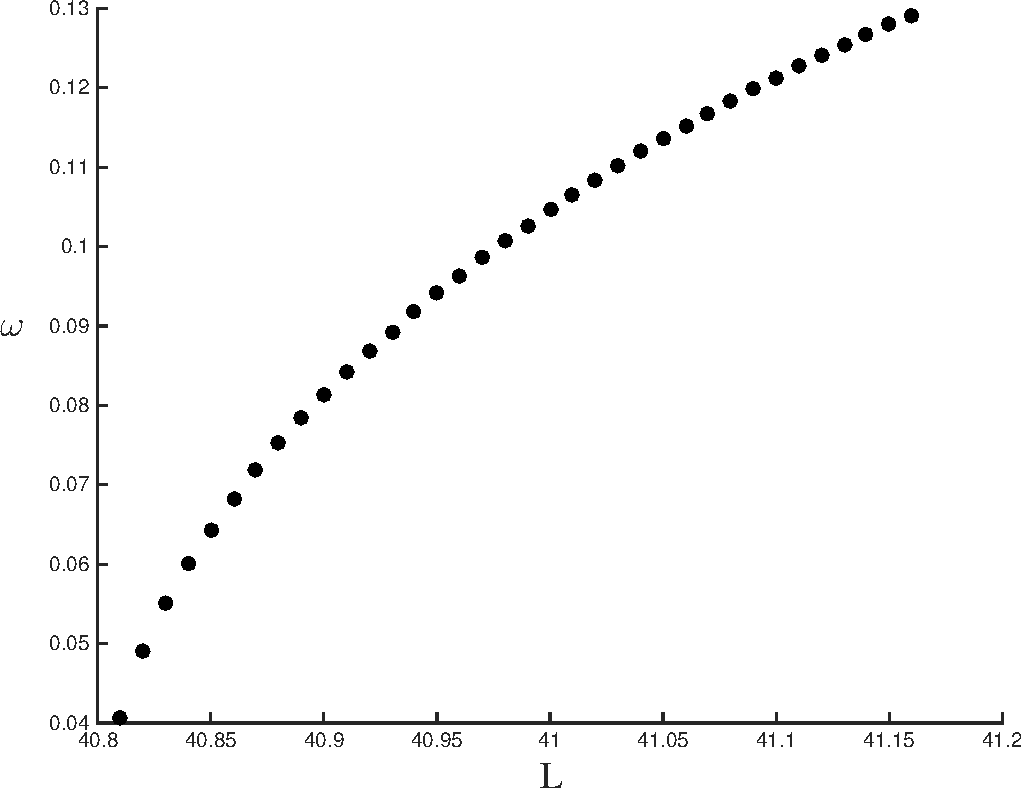
\includegraphics[width=3in]{KSRotNums2}
  \caption{
  Rotation number $\omega$ of the invariant tori of the \KSe\ for
  different system sizes $L$.  The torus does not appear vulnerable to
  resonances.
   }
  \label{fig:KSRotNums}
 \end{figure}

\section{Conclusions}
\label{s:concl}

In this paper we explored the life cycle of an invariant torus of the
Kuramoto-Sivashinsky system.  We showed that the birth and death of a
such a torus can be determined by studying the periodic orbit contained
within the interior of the torus.  We also demonstrated that the torus is
robust to resonance in the rotation number of the orbit.

As we had noted in \refsect{s:Life}, the torus we compute is narrow and
is therefore presumably of little importance for the computation of dynamical
averages.  There may be other tori in the Kuramoto-Sivashinsky system
that are larger, occupying a significant region in phase space.  These
tori could have a remarkable role in the dynamics, and appreciably
advance our understanding of these systems.  The results and methods
described in this paper will allow us to begin searching for such
consequential invariants.

\begin{acknowledgments}
The life \& death question was posed by P. Cvitanovi{\'c}, whose advice
was helpful throughout this project.
Author is also indebted to
Y. Lan
and
J.D. Meiss
for inspiring discussions.
Author acknowledges support by NSF grant DMS-1162544
and Western New England University.
\end{acknowledgments}


\bibliography{../bibtex/elton}


\ifdraft
    \onecolumngrid

    \newpage
%\input ../blog/FoxCvi14flotsam
%\input figures
\fi

%%%I don't think this is relevant for the paper but didn't want to delete it all....so its here.....
\iffalse
\section{Examples}
\subsection{Primary and secondary tori in the standard map}
As a first test we applied this method to compute both rotational and
nonrotational tori in the standard map
\begin{align}
x' & = x+ y' \mod 1\\
y' &= y+\frac{k}{2\pi} \sin(2\pi x)
\end{align}
Note that in this case $s \in [0,1]$ so an extra $2\pi$ term is needed in
the exponentials of \refeq{eq:FExp}   and \refeq{eq:Newton}.
See \reffig{fig:RotTorus} for results.

\begin{figure}%[H]
\centering
 (a) 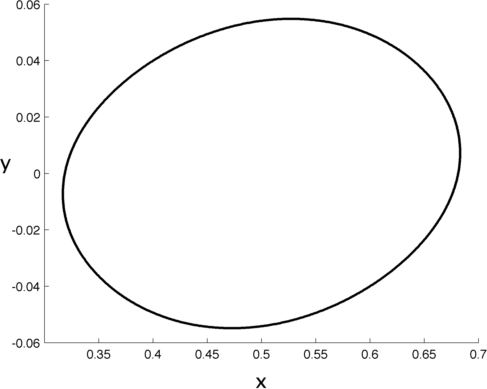
\includegraphics[width=0.45\textwidth]{NonRotTorus}
 (b) 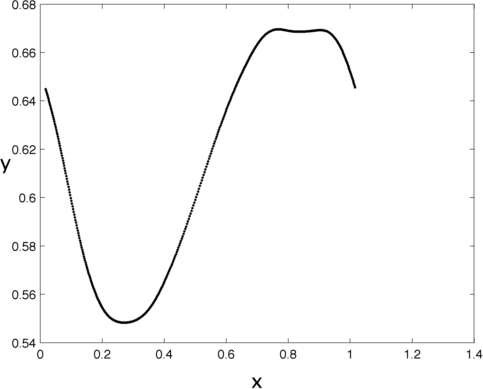
\includegraphics[width=0.45\textwidth]{RotTorus}
\caption{
Primary tori in the standard map.
(a)
$k=0.1$, $\omega=\frac{3}{40}\gamma$ (where
$\gamma$ is the golden mean). Converged to an error of 6.4e-9.
The initial guess was given by the circle of radius 0.2 centered at
(.5,0).
(b)
The $\gamma-1$ torus at $k=.75$ with
the initial condition given by the integrable $k=0$ torus.  The error is
below $10^{-15}$.  In both cases 512 modes were used, and 128 were
`kept.'
}
\label{fig:RotTorus}
\end{figure}

\subsection{Primary tori in a forced pendulum}
As a second test we explored tori in a 1.5 dof Hamiltonian system with
\begin{equation}\label{eq:Hamilton}
H(p,x,t)=\frac{p^2}{2}-\varepsilon(\cos(x)+\cos(x-t))
\eeq
where $(x,t) \in \mathbb{T}^2$.  We compute a torus by examining the stroboscopic $t=0 \mod 2\pi$ map.
The {\jacobianM} is computed by simultaneously integrating
\begin{equation}\label{eq:Jac}
\frac{dJ}{d\tau}=AJ, \hspace{.5in} J(0)=I.
\end{equation}
where $A_{jk}=d\dot{a}_j/da_k$.

The $\gamma-1$ torus at $\varepsilon=0.02$ is shown in
\reffig{fig:Snorm}\,(b), computed using 512 modes with 128 `kept.'


\subsection{Predicting criticality}
In previous studies a Sobolev seminorm has proven useful in approximating the breakdown of analyticity of tori. These studies have examined this seminorm for the conjugacy of the tori, however I theorized that it should work for the torus itself as well.

I define the Sobolov seminorm as
\begin{equation}\label{eq:Snorm}
H^k=\sum_j (2\pi j)^{2k}|a_j|^2
\end{equation}
I have been using $k=2$ since this gave the best results in my previous
work, although I should try other values as well.  I choose some initial
step size in $\eps$ and step up in
$\eps$, computing the torus at each step, requiring the final
error to be below a certain threshold.  I use quadratic interpolation to generate
guesses for the new tori.

The first time the algorithm fails to converge to the specified tolerance I decrease the step size and double the number of Fourier modes, then continue stepping up in $\eps$.  At every following failure, I double the number of Fourier modes, however keep the step size in $\eps$ fixed.  When the number of Fourier modes exceeds a specified limit the algorithm exits.  Some typical data is shown in \reffig{fig:Snorm}\,(a).

\begin{figure}%[H]
\centering
 (a) 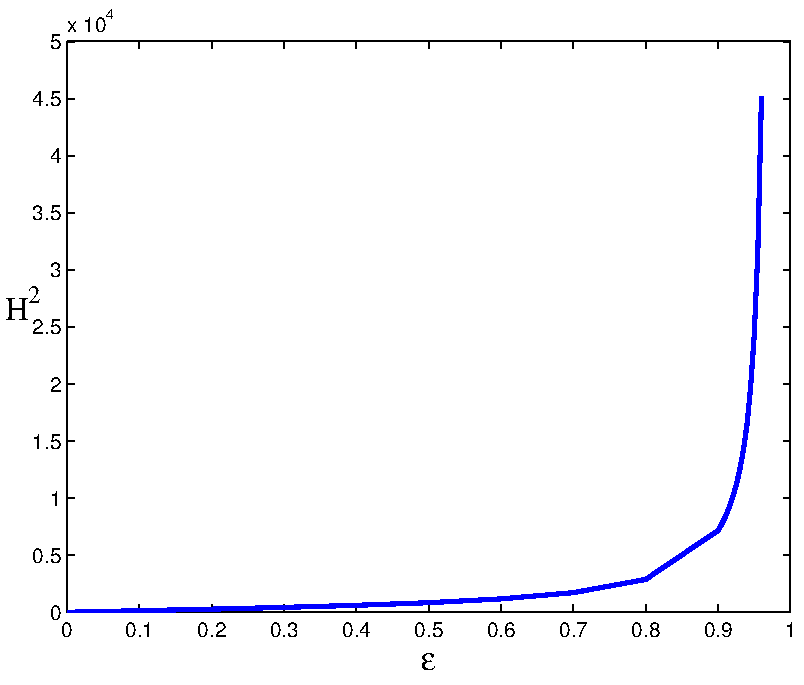
\includegraphics[width=0.45\textwidth]{Snorm}
 (b) 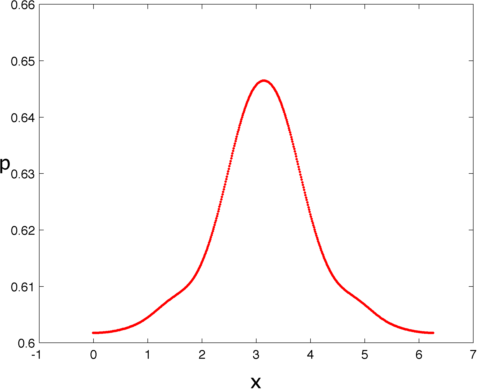
\includegraphics[width=0.45\textwidth]{PHamilRotTorus}
\caption{
(a)
Sobolev norm as a function of $\eps$ for the golden mean torus in the standard map.
(b)
Primary tori in a forced pendulum.
}
\label{fig:Snorm}
\end{figure}

I experimented with a variety of values for $M$ and $N$, and step sizes in $\varepsilon$.  The best results came from starting with $N=256$ $M=N/4$. For the standard map I set the ceiling at $N=2048$ while for the pendulum I used $N=1024$ (this choice was mainly due to time constraints).  For step sizes, I used $0.1$ and $0.005$ while for the pendulum I used $0.005$ and $0.0001$.  I required the standard map tori to be accurate to $10^{-12}$ while the pendulum tori were required to be accurate to $5\times10^{-6}$.

I took all the $(\varepsilon, H^2)$ pairs, using the action component in \refeq{eq:Snorm} and fitted them to the curve
\[
H^2=A(\varepsilon_{cr}-\varepsilon)^b.
\]
Using a 3-point fit we find that the golden mean torus of the standard map is destroyed at $\varepsilon_{cr}\approx0.97175$, so the error is $\mathcal{O}(10^{-4})$.  The same torus is destroyed at $\eps=0.027392$ for the pendulum system.  In his paper, C Chandre estimated $\varepsilon_{cr}=0.02759$, so the estimates agree to $\mathcal{O}(10^{-4})$.

This method appears to predict criticality accurately and is quite rapid.

One additional note: I do some extra anti-aliasing before computing the seminorm and interpolating to find the next guess.  I sent all modes with mode number greater than $N/8$ to zero.  I found this provided for additional numerical stability.
\fi

\end{document}
